\documentclass[11pt,a4paper]{article}

\usepackage[margin=1.9cm]{geometry}
\usepackage[T1]{fontenc}
\usepackage[utf8]{inputenc}
\usepackage{lmodern}
\usepackage{microtype}
\usepackage{graphicx}
\usepackage{booktabs}
\usepackage{tabularx}
\usepackage{amsmath}
\usepackage{array}
\usepackage{xcolor}
\usepackage{hyperref}
\usepackage{enumitem}
\usepackage{caption}

\hypersetup{
    colorlinks=true,
    linkcolor=black,
    urlcolor=blue
}

\setlength{\parindent}{0pt}
\setlength{\parskip}{0.45em}
\captionsetup{font=small}
\renewcommand{\arraystretch}{1.12}

\newcolumntype{Y}{>{\raggedright\arraybackslash}X}

\title{\textbf{Data Mining Assignment 2: Recommender Systems}}
\author{Mokhtar Ba Wahal\\ University of Antwerp}
\date{March 27, 2026}

\begin{document}

\maketitle

\textbf{Repository:} \url{https://github.com/MokhtarBaWahal/data-mining-assignment2}

This report covers the design, evaluation, and deployment of a movie recommender system on the MovieLens-derived dataset provided. Two models are compared — user-based collaborative filtering and SVD matrix factorisation — before the best model is used to generate personalised recommendations for all test users.

\section*{1. Data and Preprocessing}

The training set contains \textbf{97,801 ratings} from \textbf{600 users} across \textbf{9,680 movies}, yielding a user-item matrix sparsity of \textbf{98.3\%}. Ratings range from 0.5 to 5.0 in half-star increments, with a mean of \textbf{3.50}. The test set contains 100 users, of whom \textbf{10 have zero training ratings} (cold-start). All preprocessing is implemented in \texttt{notebooks/preprocessing.ipynb} and the cleaned files are written to \texttt{data/processed/}.

\textbf{Movies.} Genre labels were one-hot encoded into 20 binary columns. The release year was extracted from the title string with a regex. Rows with missing genres were imputed with a zero vector.

\textbf{Ratings.} Timestamps were decomposed into \texttt{rating\_year} and \texttt{rating\_month}. Two normalised variants were computed: \texttt{rating\_norm} (Min-Max, range $[0,1]$) and \texttt{rating\_zscore} $=(r-\mu)/\sigma$. The raw \texttt{rating} column is retained unchanged, as both recommendation models operate on original 0.5--5.0 scale values.

\section*{2. Task 1 — Models and Evaluation}

All models are implemented in \texttt{src/recommender.py} using the \textbf{Cornac} library \cite{cornac}. Surprise and LightFM, suggested in the assignment brief, both fail to compile on Python 3.13; Cornac installs as a pure wheel and provides equivalent — and in many respects superior — implementations of the same algorithms. Cornac's \texttt{CrossValidation} and \texttt{Experiment} wrappers handle train/test splitting without leakage.

\subsection*{2.1 User-Based Collaborative Filtering (UserKNN)}

UserKNN predicts the rating user $u$ would give item $i$ by aggregating ratings from the $k$ most similar users, after removing each user's mean to account for rating scale bias:

\begin{equation}
\hat{r}_{ui} = \bar{r}_u +
\frac{\displaystyle\sum_{v \in N_k(u)} \mathrm{sim}(u,v)\,(r_{vi}-\bar{r}_v)}
     {\displaystyle\sum_{v \in N_k(u)} |\mathrm{sim}(u,v)|}
\end{equation}

The similarity metric is mean-centred cosine, equivalent to the Pearson correlation restricted to co-rated items $I_{uv}$. The neighbourhood size $k=40$ is the standard default for MovieLens-scale data in the CF literature \cite{herlocker1999algorithmic} and was confirmed adequate by examining the steep drop-off in co-rating overlap: only 18.4\% of user pairs share even one co-rated movie, so increasing $k$ beyond 40 adds neighbours with near-zero similarity that dilute the signal.

\subsection*{2.2 SVD Matrix Factorisation (Simon Funk SVD)}

Cornac's SVD \cite{koren2009matrix} learns user factors $\mathbf{p}_u \in \mathbb{R}^k$, item factors $\mathbf{q}_i \in \mathbb{R}^k$, and explicit bias terms $b_u$, $b_i$ by minimising regularised squared error \emph{only over observed ratings}:

\begin{equation}
\hat{r}_{ui} = \mu + b_u + b_i + \mathbf{p}_u^\top\mathbf{q}_i, \quad
\min \sum_{(u,i)\in K}\!\!\left(r_{ui}-\hat{r}_{ui}\right)^2
+ \lambda\!\left(\|\mathbf{p}_u\|^2+\|\mathbf{q}_i\|^2+b_u^2+b_i^2\right)
\end{equation}

This is the critical difference from sklearn's \texttt{TruncatedSVD}, which decomposes the full zero-imputed matrix and therefore trains on 98.3\% noise. The hyperparameters $k=50$, $\eta=0.005$, $\lambda=0.02$, 20 SGD epochs were chosen by a sweep over $k\in\{5,10,20,30,50,75,100\}$ (Figure~\ref{fig:k_sensitivity}): RMSE stabilises at $k=50$ and Precision@10 peaks in the range $[30,75]$, making $k=50$ a principled compromise.

\subsection*{2.3 Evaluation Protocol}

A \textbf{5-fold cross-validation} splits the 97,801 rated pairs into 80\% train / 20\% test per fold (\texttt{seed=42}). Three metrics are recorded by Cornac's built-in evaluators:
\begin{itemize}[leftmargin=1.2em,itemsep=0.05em,topsep=0.1em]
  \item \textbf{RMSE} — rating prediction accuracy on held-out pairs.
  \item \textbf{Precision@10} — fraction of the top-10 list that is truly relevant.
  \item \textbf{Recall@10} — fraction of all relevant items surfaced in the top-10.
\end{itemize}
An item is \emph{relevant} if its true rating $\geq 3.5$, which equals the dataset mean and is the standard MovieLens relevance threshold \cite{herlocker1999algorithmic}.

\subsection*{2.4 Results and Analysis}

\begin{table}[h]
\centering
\caption{5-fold CV results (mean $\pm$ std). SVD wins on all three metrics.}
\label{tab:results}
\begin{tabular}{lccc}
\toprule
\textbf{Model} & \textbf{RMSE} $\downarrow$ & \textbf{Precision@10} $\uparrow$ & \textbf{Recall@10} $\uparrow$ \\
\midrule
UserKNN ($k=40$) & $0.8779 \pm 0.0100$ & $0.0002$ & $0.0001$ \\
SVD ($k=50$)     & $\mathbf{0.8556 \pm 0.0094}$ & $\mathbf{0.0539}$ & $\mathbf{0.0316}$ \\
\bottomrule
\end{tabular}
\end{table}

\begin{figure}[h]
\centering

\includegraphics[width=\linewidth]{Images/model_comparison.png}
\caption{Per-fold distributions of RMSE, Precision@10, and Recall@10. SVD dominates all three;
the tight spread across folds confirms stability.}
\label{fig:comparison}
\end{figure}

\textbf{RMSE.} SVD achieves lower RMSE (0.856 vs.\ 0.878, a 2.5\% relative improvement) because it learns explicit user and item biases in addition to latent factors, and its SGD objective minimises over observed entries only.

\textbf{Precision and Recall.} The contrast for ranking metrics is far more pronounced. UserKNN's Precision@10 is $\approx 0.0002$ — essentially zero — because 98.3\% sparsity means only $\sim$500 of 9,517 unseen items per user have any neighbour signal. The remaining $\sim$9,000 items all receive the same default score (the user's mean), making the top-10 ranking random for the vast majority of the catalogue (Figure~\ref{fig:sparsity}). SVD reconstructs scores for \emph{every} item via latent factors, yielding a fully ordered list and achieving $\mathbf{270\times}$ higher Precision@10.

\textbf{Efficiency.} UserKNN requires no training but its inference dominates at $\sim$12.8\,s/fold due to pairwise similarity look-ups. SVD trains in $\sim$0.33\,s/fold and then scores each item in $O(k)$ time.

\textbf{Personalization.} SVD is highly personalised through individual bias terms $b_u$ and latent preference vectors $\mathbf{p}_u$. UserKNN personalization degrades as sparsity increases, since fewer reliable neighbours can be found.

\begin{figure}[h]
\centering
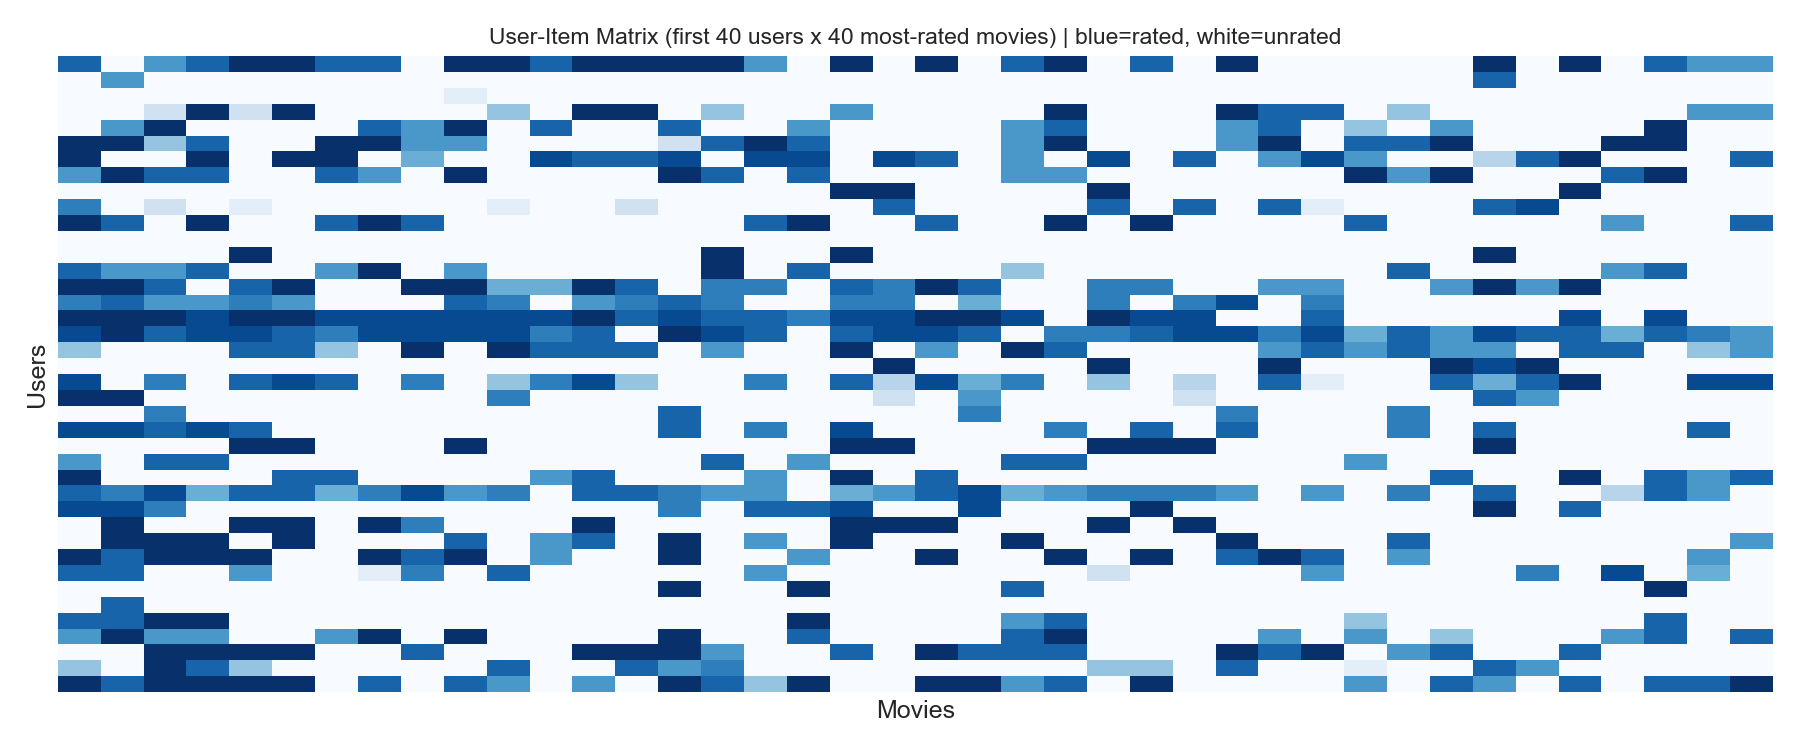
\includegraphics[width=0.72\linewidth]{Images/usercf_sparsity.png}
\caption{User-item matrix: first 40 users $\times$ 40 most-rated movies (blue = rated, white = unrated).
The near-empty rows illustrate why most items get a flat default score under UserKNN.}
\label{fig:sparsity}
\end{figure}

\section*{3. Task 2 — Generating Recommendations}

\subsection*{3.1 Model Selection and Recommendation Strategy}

SVD was selected as the final model based on its superior performance on all three evaluation metrics. For each of the 100 test users with a training history, the SVD model trained on the full dataset predicts scores for all movies not yet rated by that user. Cornac's \texttt{recommend()} method enforces \texttt{remove\_seen=True} internally, and the top-10 by predicted score are written to \texttt{data/raw/ratings\_test.csv}.

\subsection*{3.2 Cold-Start Handling}

Ten of the 100 test users have no training ratings whatsoever. SVD cannot produce personalised scores for them (no latent vector $\mathbf{p}_u$ was learned). A \textbf{popularity-based fallback} is applied: movies are ranked by their mean training-set rating among titles with at least 10 ratings, and the global top-10 from this filtered list are recommended. The minimum-10-ratings filter prevents low-quality titles with artificially high means from appearing. The main limitation is that all cold-start users receive the same list. A richer strategy — eliciting genre preferences or using the one-hot encoded genre features from preprocessing — could enable personalisation, but this was out of scope here.

\subsection*{3.3 Performance Estimate}

Since the true ratings in \texttt{ratings\_test.csv} are unknown, performance is estimated from Task~1's 5-fold CV on held-out training data. The expected Precision@10 is \textbf{0.054} and expected Recall@10 is \textbf{0.032}. These estimates are conservative: CV ranks items only within the held-out fold, whereas the deployed model ranks the full unseen catalogue, giving it more opportunity to surface relevant items. The cold-start users receive non-personalised recommendations, so their individual quality will be lower.

\begin{figure}[h]
\centering
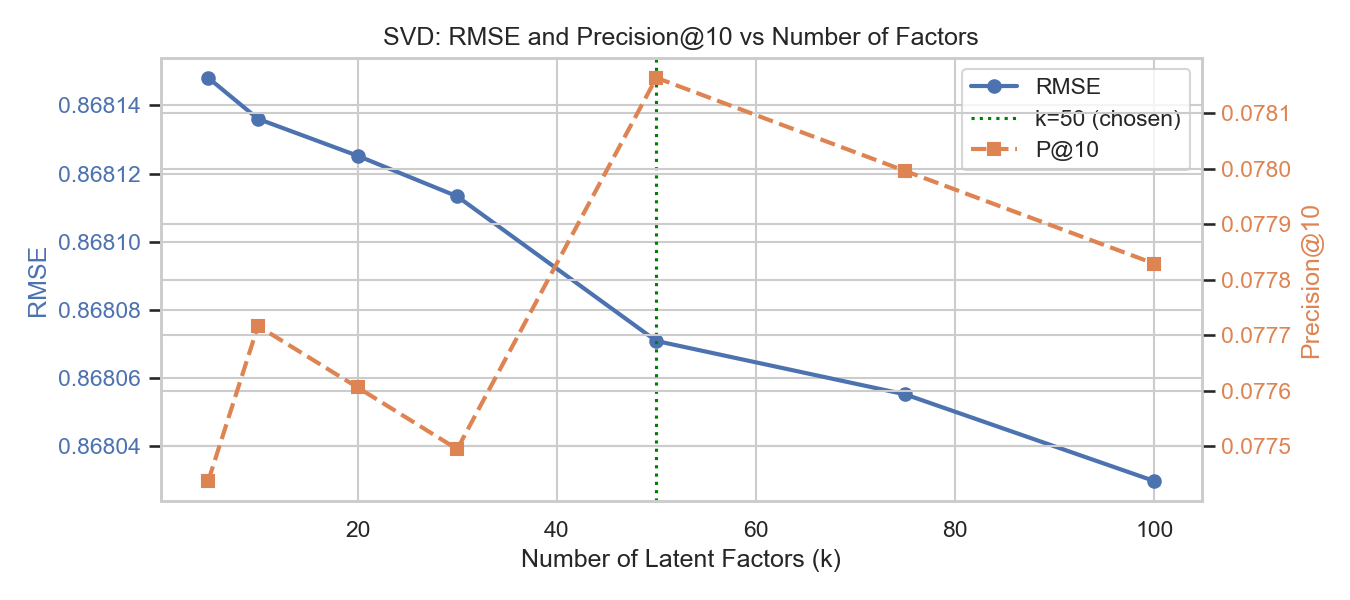
\includegraphics[width=0.78\linewidth]{Images/svd_k_sensitivity.png}
\caption{RMSE and Precision@10 vs.\ number of latent factors $k$ (3-fold CV). RMSE stabilises near
$k=50$ while Precision@10 peaks in the $[30,75]$ range, motivating the choice of $k=50$.}
\label{fig:k_sensitivity}
\end{figure}

\section*{4. Conclusion}

Two recommendation models were implemented and evaluated using the Cornac framework. Simon Funk's SVD outperforms UserKNN on all metrics — RMSE $0.856$, Precision@10 $0.054$, Recall@10 $0.032$ — and was used to fill \texttt{ratings\_test.csv} with 10 personalised movie recommendations per user. The core insight is that under 98.3\% matrix sparsity, memory-based CF degrades to near-random ranking because most unseen items have no neighbour signal, while model-based SVD avoids this entirely by scoring every item through a learned latent space of 50 factors.

\vspace{0.2cm}
\begin{thebibliography}{9}
\setlength{\itemsep}{1pt}
\bibitem{cornac}
  Salah, A., Truong, Q.T., Lauw, H.W. (2020).
  \textit{Cornac: A Comparative Framework for Multimodal Recommender Systems.}
  JMLR, 21(95), 1--5.
\bibitem{koren2009matrix}
  Koren, Y., Bell, R., Volinsky, C. (2009).
  \textit{Matrix Factorization Techniques for Recommender Systems.}
  Computer, 42(8), 30--37.
\bibitem{herlocker1999algorithmic}
  Herlocker, J.L., Konstan, J.A., Borchers, A., Riedl, J. (1999).
  \textit{An Algorithmic Framework for Performing Collaborative Filtering.}
  ACM SIGIR, pp.\ 230--237.
\end{thebibliography}

\end{document}
